\input{../preamble.tex}

\SetDate[12/03/2026]

\begin{document}
\pagestyle{fancy}
\fancyhead[L]{Tle STMG}
\fancyhead[C]{\textbf{Statistiques à deux variables}}
\fancyhead[R]{\today}

\exemulticols{}{
	Deux ajustements affines sont proposés pour approximer le jeu de données ci-contre :
		\begin{align*}
			f(x) = x + 1, && \et && g(x) = 1,2x.
		\end{align*}
	\begin{enumerate}
		\item
		À quelle droite correspond la fonction $f$ ? et $g$ ?
		\item
		Quel ajustement permet de mieux décrire les données ?
		Calculer l'erreur commise par chaque ajustement affine proposé à l'aide du tableau.
	\end{enumerate}
	\vfill
}{
	\null\vspace{-40pt}
	\begin{center}
	\begin{tikzpicture}
		\begin{axis}[xmin = 0, ymin=0, axis line style=->, extra y ticks={0}, extra x ticks={0}]
			\addplot[only marks, GREEN_E, mark size=2pt]  coordinates {(1,2)(3,3)(4,5)(4,4)(5,6)(6,5)(6,10)}; 
			
			\addplot[very thick, dashed, BLUE_E] expression[domain=0:7, samples=2]{x+1};% node[right]{$\C_f$};
			\addplot[very thick, dashed, RED_E] expression[domain=0:7, samples=2]{1.2*x} ;%node[right]{$\C_g$};
		\end{axis}
	\end{tikzpicture}
	\end{center}
}{exe:l2-comparison}{
}
	\begin{center}
\def\arraystretch{1.3}
\setlength\tabcolsep{20pt}
	\begin{tabular}{|*{8}{c|}}\hline
		$x$ & 1 & 3 & 4 & 4 & 5 & 6 & 6
		\\\hline
		$y$ & 2 & 3 & 5 & 4 & 6 & 5 & 10
		\\\hline
		$\bigl[f(x)-y\bigr]^2$ & & & & & & &
		\\\hline
		$\bigl[g(x)-y\bigr]^2$ & & & & & & &
		\\\hline
	\end{tabular}
	\end{center}

\exe{}{
	Pour chaque jeu de données de la figure \ref{fig:1}, un ajustement affine est-il pertinent ? Justifier.
}{exe:pertinentYN}{

}

\begin{figure}[h!]
\newcommand{\scale}{.9}
	\begin{subfigure}{.5\textwidth}
	\begin{tikzpicture}[scale=\scale]
		\begin{axis}[xmin = -1, xmax=13, xlabel = Ancienneté, ylabel = Salaire net, ylabel near ticks, xlabel near ticks]
			\addplot[only marks, ORANGE, mark size=2pt] table {data/entreprise-anc-sal.dat};
		\end{axis}
	\end{tikzpicture}
	\end{subfigure}
	\begin{subfigure}{.5\textwidth}
	\begin{tikzpicture}[scale=\scale]
		\begin{axis}[xmin = -.5, xmax=5.5, xlabel = Années de formation ou d'étude, ylabel = Salaire net, ylabel near ticks, xlabel near ticks]
			\addplot[only marks, ORANGE, mark size=2pt] table[x=apbac, y=sal] {data/entreprise-apbac-sal.dat};
		\end{axis}
	\end{tikzpicture}
	\end{subfigure}
	
	\begin{subfigure}{.5\textwidth}
	\begin{tikzpicture}[scale=\scale]
		\begin{axis}[xmin = -1, xmax=13, xlabel = Ancienneté, ylabel = Salaire net, ylabel near ticks, xlabel near ticks, scaled y ticks=false]
			\addplot[only marks, ORANGE, mark size=2pt] table[x=anc, y=sal] {data/entreprise-anc-sal.dat};
			\addplot[only marks, RED_E, mark size=2pt] table[x=anc, y=sal] {data/entreprise-anc-sal-CEO.dat};
			\addplot[only marks, ORANGE, mark size=2pt] table[x=anc, y=sal] {data/entreprise-anc-sal-CEO-neveu.dat};
			\addplot[only marks, ORANGE, mark size=2pt] table[x=anc, y=sal] {data/entreprise-anc-sal-esclave.dat};
			
			%\addplot[thick, dashed, BLUE_E] expression[domain=0:12, samples=2]{1100 + 700*x};
		\end{axis}
	\end{tikzpicture}
	\end{subfigure}
	\begin{subfigure}{.5\textwidth}
	\begin{tikzpicture}[scale=\scale]
		\begin{axis}[xmin = -.5, xmax=5.5, ymin=900, ymax=2100, xlabel = Ancienneté, ylabel = Salaire net, ylabel near ticks, xlabel near ticks]
			\addplot[only marks, ORANGE, mark size=2pt] table[x=anc, y=sal] {data/entreprise-anc-sal-fewpoints.dat};
			%\addplot[very thick, dashed, BLUE_E] expression[domain=0:5, samples=2]{950 + 150*x};
			%\addplot[very thick, dashed, RED_E] expression[domain=0:5, samples=2]{2050 - 150*x};
		\end{axis}
	\end{tikzpicture}
	\end{subfigure}
%	\begin{subfigure}{.2\textwidth}
%	\begin{tikzpicture}
%		\begin{axis}[xmin = -.5, xmax=13, xlabel = Ancienneté, ylabel = Salaire net, ylabel near ticks]
%			\addplot[only marks, ORANGE, mark size=2pt] table[x=anc, y=sal] {data/entreprise-anc-sal-quadratic.dat};
%			\addplot[very thick, BLUE_E] expression[domain=0:5, samples=2]{1100 + 250*x};
%			\addplot[very thick, dashed, BLUE_E] expression[domain=5:12, samples=2]{1100 + 250*x};
%		\end{axis}
%	\end{tikzpicture}
%	\end{subfigure}
	\caption{Figures de l'exercice \ref{exe:pertinentYN}.}
	\label{fig:1}
\end{figure}


\newpage


\exemulticols{, difficulty=1}{
	Soient $f(x) = ax+b$ et $g(x) = a'x+b'$ deux fonctions affines données graphiquement pour $3,2 \leq x \leq 3,7$ ci-contre.
	
	\begin{enumerate}
		\item
		Pour chaque droite, donner deux points $A$ et $B$ lui appartenant.
		\item
		Déterminer les paramètres $a, b, a',$ et $b'$.
	\end{enumerate}
	
	\vfill
	
	\emph{Formules :}
	\begin{align*}
		a = \dfrac{y_B-y_A}{x_B-x_A} && \et && b =y_A - ax_A
	\end{align*}
	
	%\vfill\null
}{
	\begin{center}
	\begin{tikzpicture}[>=stealth, scale=.8]
	\begin{axis}[xmin = 3.2, xmax=3.7, ymin=5, ymax=7, axis x line=middle, axis y line=middle, axis line style=->, xtick distance=.1, ytick distance = 1,  enlargelimits=.1, grid=both, clip=true, minor x tick num = 1, minor y tick num = 3, x=500pt]
		
		% Cf
		\addplot[BLUE_E, very thick, domain =3.2:3.7, samples=2] {-1+2*x}  node[pos = .9, above left] {$\C_f$};
		\addplot[BLUE_E, very thick, dashed, domain =3.1:3.2, samples=2] {-1+2*x} ;
		\addplot[BLUE_E, very thick, dashed, domain =3.7:3.8, samples=2] {-1+2*x};
		
		% Cg
		\addplot[RED_E, very thick, domain =3.2:3.7, samples=2] {13-2*x}  node[pos = .9, below left] {$\C_g$};
		\addplot[RED_E, very thick, dashed, domain =3.1:3.2, samples=2] {13-2*x};
		\addplot[RED_E, very thick, dashed, domain =3.7:3.8, samples=2] {13-2*x};
	\end{axis}
	\end{tikzpicture}
	\end{center}
}{exe:extrapolation-graphique1}{
	Cherchons d'abord $a$ et $b$, paramètres de la fonction affine $f$.
	
	\underline{Calcul de $a$}
	
	En connaissant deux points $A$ et $B$ de $\C_f$, on peut immédiatement déduire un vecteur directeur (par exemple $\vec{AB}$) et le coefficient directeur de $f$.
	D'après le cours, ceci est équivalent à calculer 
		\[ a = \dfrac{y_B - y_A}{x_B - x_A}, \]
	mais gardons la méthode vectorielle qui scinde les calculs en plusieurs parties.
	
	Graphiquement, on lit $A(3,25 ; 5,5)$ et $B(3,5 ; 6)$, desquel on déduit
		\[ \vec{AB} = \pvec{3,5-3,25}{6-5,5} = \pvec{0,25}{0,5} = 0,25 \pvec{1}{\frac{0,5}{0,25}} = 0,375 \pvec{1}{2}. \]
	Par conséquent, $a = 2$.
	
	\underline{Calcul de $b$}
	
	Nous ne disposons pas de point d'abscisse nulle duquel lire l'ordonnée à l'origine simplement.
	Cependant, comme $a =2$, nous savons que $f(x) = 2x+b$.
	De plus, comme $A\in\C_f$, nous pouvons obtenir la relation $y_A = f(x_A)$, qui n'admet qu'une seule inconnue, $b$, et qui permet donc de trouver la valeur de l'ordonnée à l'origine.
	\begin{align*}
		y_A = 5,5 &= f(x_A) \\
					&= f(3,25) \\
					&= 2\cdot3,25 + b \\
					&= 6,5 + b
	\end{align*}
	Il suit donc que $5,5 = 6,5+b$ et donc que $b = 5,5-6,5 = -1$.
	
	Notons, pour nous convaincre que notre choix arbitraire de point n'influe pas le résultat, que le même raisonnement avec $B\in\C_f$ donne le même résultat :
	\begin{align*}
		y_B = 6 &= f(x_B), \\
					&= f(3,5), \\
					&= 2\cdot3,5 + b, \\
					&= 7 + b.
	\end{align*}
	Par suite, $b = 6-7 = -1$.
	
	Nous concluons que $f(x) = 2x - 1$.
	
	
	En procédant similairement, nous obtenons $g(x) = -2x + 13$. (Ou $13-2x$ si on cherche à minimiser l'encre utilisée pour écrire l'expression.)
}



\exe{}{
	Une entreprise décide de mettre un nouveau produit sur le marché. Pour déterminer son prix de vente, elle réalise plusieurs tours
	de vente limités en faisant varier le prix unitaire. Les résultats obtenus sont donnés dans le tableau ci-dessous.
	
	\begin{multicols}{2}
	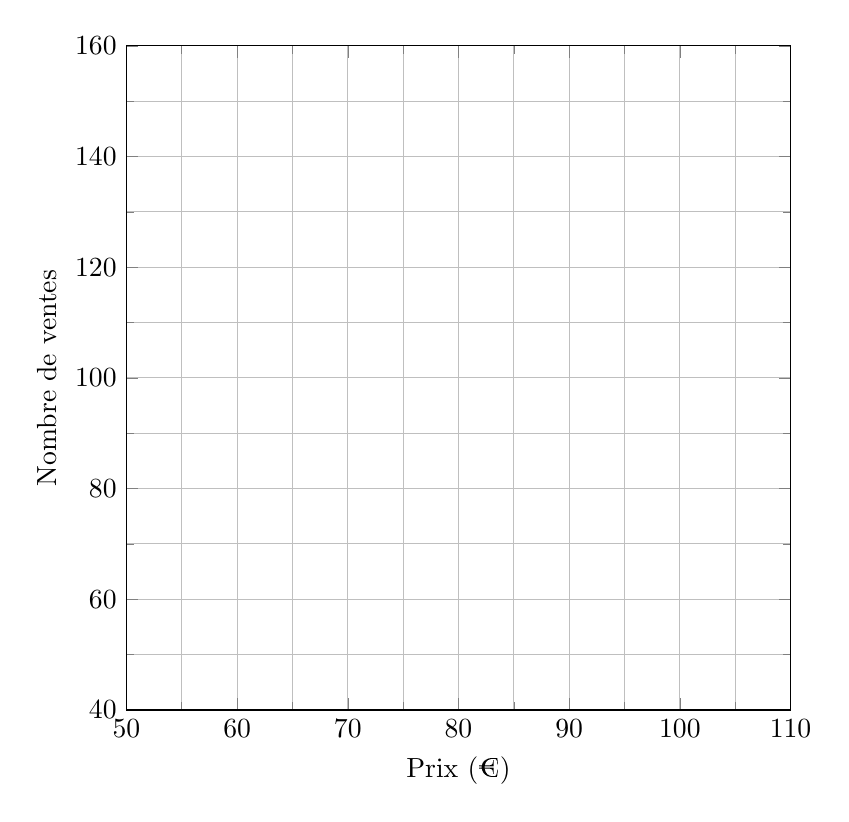
\begin{tikzpicture}
	\begin{axis}[
 		axis line style=->,
		grid=both,
		minor tick num=1,
		xtick distance=10,
		ytick distance=20,
		x=4pt,
		y=2pt,
		xmin=50,
		xmax=110,
		ymin=40,
		ymax=160,
		xlabel = Prix (€),
		ylabel = Nombre de ventes,
		ylabel near ticks,
		xlabel near ticks,
		clip=true,
		]
		%\addplot[only marks, BLUE_E, mark size=2pt]  coordinates {(50,150)(55,138)(60,130)(80,92)(100,48)}; 
	\end{axis}
	\end{tikzpicture}
\def\arraystretch{2}
\setlength\tabcolsep{10pt}
	\null\hfill
	\begin{tabular}{|c|c|c|}
		\hline
		\textbf{Prix} & \textbf{Ventes} & \textbf{Recettes}
		\\\hline
		50 & 150 & \\ \hline
		55 & 138 & \\ \hline
		60 & 130 & \\\hline
		65 &  & \\\hline
		70 &  & \\\hline
		75 &  & \\\hline
		80 & 92 & \\ \hline
		90 &  & \\\hline
		100 & 48 & \\\hline
	\end{tabular}
	\vfill\null
	\end{multicols}
	
	\begin{enumerate}
		\item
		Représenter les données du tableau dans le repère ci-dessus.
		\item 
		Déterminer l'équation d'une droite $(d)$ d'ajustement affine liant le nombre de ventes $y$ et le prix $x$ sous la forme $y=ax+b$.
		Arrondir les paramètres $a$ et $b$ à l'unité.
		\item 
		À l'aide de cet ajustement affine, remplir la colonne « Ventes » du tableau.
		\item 
		Selon vous, quel est le prix permettant à l'entreprise de réaliser le plus grand chiffre d'affaire ?
		Remplir la colonne « Recettes » du tableau pour répondre à la question.
	\end{enumerate}
 
}{exe:recettes}{
	\begin{center}
	\begin{tikzpicture}
	\begin{axis}[
 		axis line style=->,
		grid=both,
		minor tick num=1,
		xtick distance=10,
		ytick distance=20,
		x=4pt,
		y=2pt,
		xmin=50,
		xmax=110,
		ymin=40,
		ymax=160,
		xlabel = Prix (€),
		ylabel = Nombre de ventes,
		ylabel near ticks,
		xlabel near ticks,
		clip=true,
		]
		\addplot[only marks, BLUE_E, mark size=2pt]  coordinates {(50,150)(55,138)(60,130)(80,92)(100,48)}; 
	\end{axis}
	\end{tikzpicture}
	\end{center}
}

\newpage

\exe{}{
	La coopérative de Mai à Clermont-Ferrand décide de mesurer le volume sonore lors des concerts qu'elle organise sur un trimestre.
	Pour cela, deux variables sont mesurées :
	\begin{enumerate}[label=(\roman*)]
		\item la pression accoustique (exprimée en pascals Pa) ;
		\item le niveau d'intensité sonore du bruit (exprimée en décibels dB).
	\end{enumerate}
	Les résultats obtenus sont présentés dans le tableau ci-dessous.
	 
	 
	\begin{multicols}{2}
		\begin{center}
		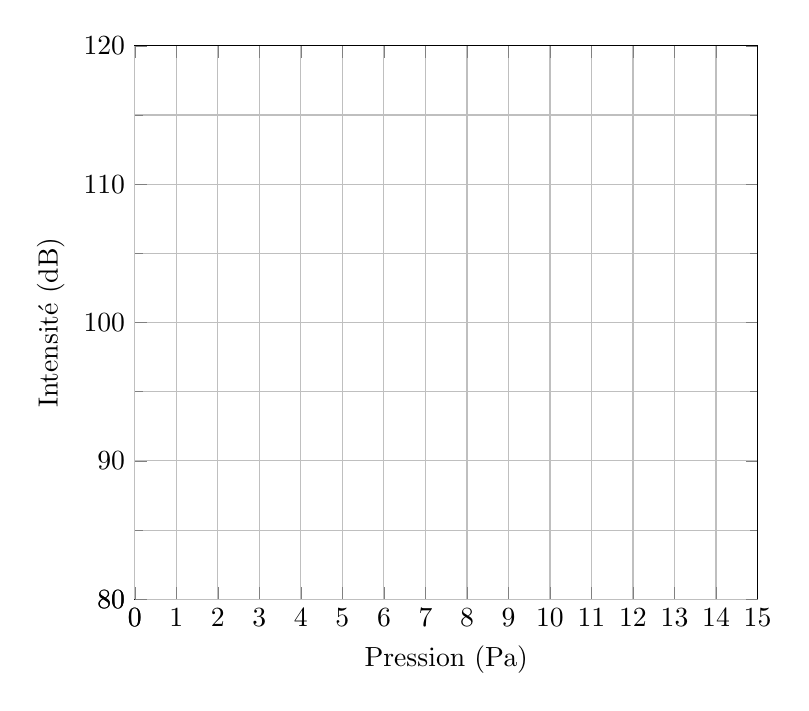
\begin{tikzpicture}
		\begin{axis}[
	 		axis line style=->,
			grid=both,
			minor y tick num=1,
			xtick distance=1,
			ytick distance=10,
			extra x ticks={0},
			extra y ticks={80},
			x=15pt,
			y=5pt,
			xmin=0,
			xmax=15,
			ymin=80,
			ymax=120,
			xlabel = Pression (Pa),
			ylabel = Intensité (dB),
			ylabel near ticks,
			xlabel near ticks,
			clip=true,
			]
		%\addplot[only marks, BLUE_E, mark size=2pt]  coordinates {(.5,88)(1,94)(3,103)(5,108)(7,111)(10,114)(13,116)(15,117)}; 
		\end{axis}
		\end{tikzpicture}
		\end{center}
\def\arraystretch{2}
\setlength\tabcolsep{5pt}
	\null\hfill
	\begin{tabular}{|c|c|c|}
		\hline
		\textbf{Pression} & \textbf{Intensité} & \textbf{LogPression}
		\\\hline
		0.5 & 88 & \\ \hline
		1 & 94 & \\ \hline
		3 & 103 & \\\hline
		5 & 108 & \\\hline
		7 & 111 & \\\hline
		10 & 114 & \\\hline
		13 & 116 & \\ \hline
		15 & 117 & \\\hline
	\end{tabular}
	\vfill\null
	\end{multicols}
	
	\begin{enumerate}
		\item
		Un ajustement affine des données vous semble-t-il pertinent ? Justifier.
		\item
		On propose de réaliser une transformation logarithmique de la pression en lui appliquant le logarithme.
		Compléter le tableau arrondissant les logarithmes à $10^{-1}$ près.
		\item
		Représenter le nouveau nuage de points dans le repère ci-dessous.
		\item 
		Déterminer l'équation d'une droite $(d)$ d'ajustement affine liant l'intensité $y$ et la logpression $\log(x)$ sous la forme $y=a\log(x)+b$.
		Arrondir les paramètres $a$ et $b$ à l'unité.
		\item
		Lors d'un concert de LuLu, artiste clermontois, l'oreille d'un spectateur est soumise à une pression de 130 Pa. 
		Estimer l'intensité sonore atteinte lors de ce concert au décibel près.
	\end{enumerate}
	
	
	\begin{center}
	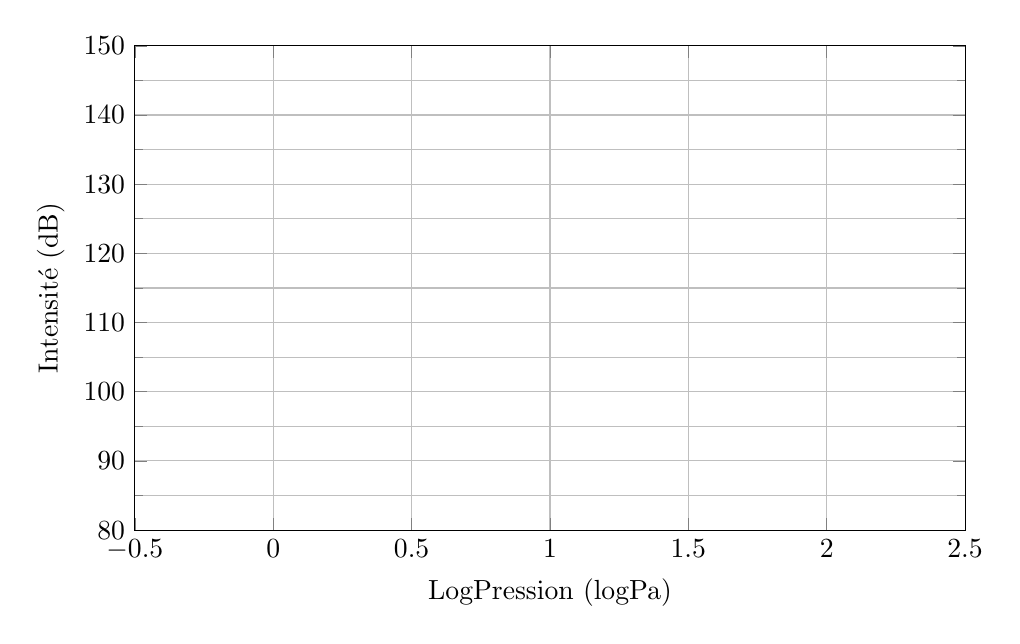
\begin{tikzpicture}
	\begin{axis}[
 		axis line style=->,
		grid=both,
		minor y tick num=1,
		%xtick distance=1,
		ytick distance=10,
		%extra x ticks={0},
		%extra y ticks={80},
		x=100pt,
		y=2.5pt,
		xmin=-.5,
		xmax=2.5,
		ymin=80,
		ymax=150,
		xlabel = LogPression (logPa),
		ylabel = Intensité (dB),
		%ylabel near ticks,
		xlabel near ticks,
		clip=true,
		]
		%\addplot[only marks, ORANGE, mark size=2pt]  coordinates {(-.3,88)(0,94)(.48,103)(.7,108)(.84,111)(1,114)(1.11,116)(1.17,117)}; 
	\end{axis}
	\end{tikzpicture}
	\end{center}
	
	
	
}{exe:LuLu}{

		\begin{center}
		\begin{tikzpicture}
		\begin{axis}[
	 		axis line style=->,
			grid=both,
			minor y tick num=1,
			xtick distance=1,
			ytick distance=10,
			extra x ticks={0},
			extra y ticks={80},
			x=15pt,
			y=5pt,
			xmin=0,
			xmax=15,
			ymin=80,
			ymax=120,
			xlabel = Pression (Pa),
			ylabel = Intensité (dB),
			ylabel near ticks,
			xlabel near ticks,
			clip=true,
			]
		\addplot[only marks, BLUE_E, mark size=2pt]  coordinates {(.5,88)(1,94)(3,103)(5,108)(7,111)(10,114)(13,116)(15,117)}; 
		\end{axis}
		\end{tikzpicture}
		
		
	\begin{tikzpicture}
	\begin{axis}[
 		axis line style=->,
		grid=both,
		minor y tick num=1,
		%xtick distance=1,
		ytick distance=10,
		%extra x ticks={0},
		%extra y ticks={80},
		x=100pt,
		y=2.5pt,
		xmin=-.5,
		xmax=2.5,
		ymin=80,
		ymax=150,
		xlabel = LogPression (logPa),
		ylabel = Intensité (dB),
		%ylabel near ticks,
		xlabel near ticks,
		clip=true,
		]
		\addplot[only marks, ORANGE, mark size=2pt]  coordinates {(-.3,88)(0,94)(.48,103)(.7,108)(.84,111)(1,114)(1.11,116)(1.17,117)}; 
	\end{axis}
	\end{tikzpicture}
		\end{center}
}




%%%%%%%%%%%%

\newpage
\fancyhead[C]{\textbf{Solutions}}
\shipoutAnswer

\end{document}
